\chapter{从团队实验到持续改善} % Introduction chapter suppressed from the table of contents



冲刺回顾是团队分析根因在下一轮冲刺改进的最佳时机，前面介绍了时间表(Timeline)，颜色点等方法收集团队“软”数据，这章会针对“硬”数据。如果团队了解改正(Correction)和 纠正措施(Corrective Action)的区别，和根因分析，便可用在回顾时分析数据，制定有效纠正措施，避免发生过的问题再发生。

\hypertarget{ux6536ux96c6ux54eaux4e9bux6570ux636e}{%
\subsection{收集哪些数据}\label{ux6536ux96c6ux54eaux4e9bux6570ux636e}}

\hypertarget{ux7f8eux56fdux67d0ux5bb6ux533bux9662ux7684ux6545ux4e8b}{%
\subsubsection{美国某家医院的故事}\label{ux7f8eux56fdux67d0ux5bb6ux533bux9662ux7684ux6545ux4e8b}}

1996年，某家美国Cook
County医院做了个试验。这家医院所在的地区比较穷困，很多市民没有买医疗保险，且医院床位紧张。因人口老化，也没有良好饮食习惯，这医院面对的最大问题是怎么判断病人有没有急性心脏病的危险？
因为如果病人胸口痛，医生从他的背景、年龄、生活习惯判断有心脏病的危险，就要收他住院，但医院的床位有限。
新来的院长Reilly很有经验，了解问题严重，首先要解决这个难题，因为针对心脏病的治疗的病床要花费2000美元一晚，一般心脏病要住3晚，而后面发现很多病人其实没有心脏病，浪费了医院的宝贵资源。
他发现每个医生都会有自己的一套方式去判断病人是否需要住院，诊断的差异很大。每个医生要收集的数据也很多，心电图、血液、尿液、x光，还有病人的历史、习惯等。
因为院长是从东岸名牌医院过来的。他认识专家专门研究怎么有效去判断病人的专家。这位专家Goldman用了两年时间，针对心脏病猝死的诊断，收集了很多数据和验证，发现只需要针对3个紧急的风险因素，就可以准确判断：

\begin{enumerate}
\tightlist
\item
  病人的肺部有没有液体
\item
  血压上压(systolic Blood pressure)是否低于100
\item
  病人是否感到心绞痛 (patient unstable angina)
\end{enumerate}

通过这样就可以判断病人是否需要住院。所以院长就依据这个做了实验。结果发现，平常用以前的方式，医生诊断准确度只有75\%-85\%，但用了这个准确度就超过95\%。\\
很多人都误解度量分析必须像大数据分析一样，要有大量数据，用很多因子来求出一个漂亮的方程式，才算成功。其实是反过来，如果想要收集的数据量越大，变量越多，量化过程改进越难成功，开发人员越抵触。所以我们必须要针对想改进的重点收集对应数据。

很多时候信息量多，但是没有针对性，反而不好。

好比病人去医院，都必须抽血、验尿、做心电图，收集各类数据让医生诊断，但是否信息越多越齐全就越好。从上面美国Cook
County医院的故事看到其实不是，

小时候看病，中医是用望闻问切的方式；西医就是用听诊器听心跳、呼吸，看舌头、口腔，然后也是听你的问题描述，便可以诊断开药了。现在去医院排队看病，医生第一件事就给你开四五张各类的检查单，通过这些检查报告做诊断。虽然我是外行，但我觉得小时候那种不超过十分钟诊断过程不会比现代的起码两个小时的诊断质量差。''\\
===如何建立并完善缺陷预测模型的例子===
公司度量分析人员展示了一个大表，上面密密麻麻有五、六十个项目变量，包括缺陷、进度、工作量等等。\\
我问：为什么你们要收集这么多数据量？你们的改进目标是什么？\\
度量分析人员：我们要提高生产率、减少进度偏差，也要降低最终的客户的缺陷密度。\\
我问:
如能尽早发现缺陷，加强前面的评审效率来减少遗漏到后面的缺陷，减少返工。如果大家都相信这可行，就应该专注这模型相关的度量，如每迭代的缺陷分布、与相关返工工作量等，让蒙地卡罗预测模型可以尽快跑起来。但如果对进度偏差，工作量偏差等都要收集，每轮可能要收集几十个变量，反而没有针对性。\\
我们看看这预测缺陷模型，比如你们有什么不同的评审方式？效果有什么不同？\\
度量分析人员：我们跟开发讨论过，确实有些区分，例如，如果我们在前期有做正式评审，质量都会好一些，但是如果没有的话，后面确实缺陷就多了。如果我们有明确需求，例如按活动、实体方式明确写出来，跟没有的话也会有质量的区分。有些项目有规定要静态扫描代码并记录缺陷，后期的缺陷数会较少。\\
我总结说:
所以如果可以估计各种方式的缺陷排除率/引入缺陷率,便可使用模型预测最终会遗漏多少缺陷。
可利用这蒙地卡罗预测工具，帮你比较各种方法，制定缺陷数目标。团队开始时先参考上一轮迭代数据，估一下预测模型参数，并一起头脑风暴讨论有什么新方法可以做提升，加进模型，蒙地卡罗预测模型可比较不同的组合，看看对缺陷率，缺陷排除率和工作量等有什么影响，团队便可参考模型的建议，最终选择下一迭代的配搭。\\
例如有些团队利用静态代码扫描预先找出代码缺陷，就可以做个实验，区分一下是否代码扫描后，系统测试缺陷会减少，排除缺陷的百分比是多少等。\\
开始的时候可能数据量不多，慢慢项目多了数据也可以看是否稳定，便开始变成团队的基线。所以开始时不要太计较准不准，而是尽快利用这概念开始量化管理。\\
如果团队能尽早发现缺陷并修复，后面返工量便可倍数降低，生产率自然也会提升，进度偏差也会改善。所以建议只针对能如何尽早发现并解决缺陷，减少返工工作量设定目标，量化管理。

\hypertarget{ux7f3aux9677ux6392ux9664ux7387}{%
\subsection{缺陷排除率}\label{ux7f3aux9677ux6392ux9664ux7387}}

从需求到设计、编码、单元测试、系统测试、验收，整个开发过程大家都很熟悉，需求、设计、编码后可以通过评审来排除缺陷，但仅仅做评审不一定能确保质量。因为最终验收缺陷数取决于每个步骤能否有效排除当前的缺陷。

可用缺陷排除率(Defect Removal Efficiency DRE) 来判断每一个过程的质量：\\
%\href{文件:jalote_emm_7.1-1.jpg}{500px}

\includegraphics[width=10cm]{jalote_emm_71-1.jpg}

图13-1

%\href{文件:Ma3_1.0.png}{文件:Ma3 1.0.png}

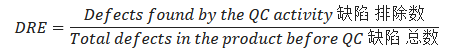
\includegraphics[width=10cm]{Ma3_10.png}

如果要最终质量好，缺陷排除率就要高。但计算缺陷排除率，必须要等到整个开发完成才可以计算。

\hypertarget{ux7f3aux9677ux6392ux9664ux9884ux6d4bux6a21ux578bux5b9eux4f8b}{%
\subsection{缺陷排除预测模型实例}\label{ux7f3aux9677ux6392ux9664ux9884ux6d4bux6a21ux578bux5b9eux4f8b}}

\begin{itemize}
\tightlist
\item
  团队分析迭代缺陷数据，缺陷是源自需求/设计/编码，得出以下分布表：\\
\end{itemize}

%\url{文件:微信截图_20220316093044.jpg}

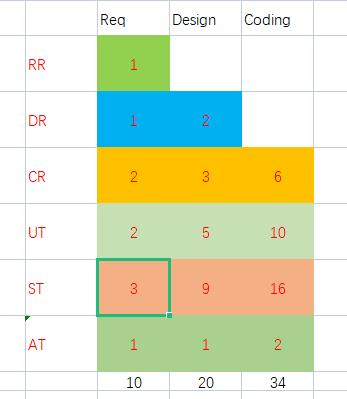
\includegraphics[width=10cm]{微信截图_20220316093044.jpg}

图13-2

A/按缺陷排除率(DRE)公式，计算出各个过程的缺陷排除率，并把参数输进水晶球模型。例如第一行Quality那行：在底栋填
10 (共有10个缺陷是源自需求）；第二行：在第4栋填 10\%
(需求评审缺陷排除率是10\%）。(本来迭代缺陷参数都标Infosys 识别。)


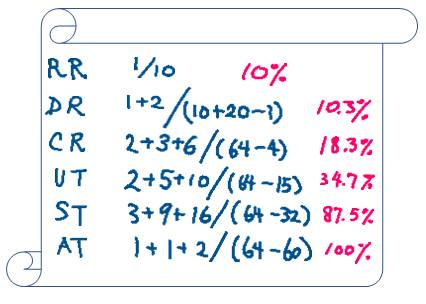
\includegraphics[width=10cm]{2DreEstimateScreenshot_2021-12-01_2120491.jpg}

图13-3


B/ 按以上迭代回顾缺陷分析结果，按以下输入框位置输进模板

\begin{enumerate}
\tightlist
\item
  需求引入缺陷数=10（3）
\item
  需求评审缺陷排除率= 10\%（4）
\item
  设计引入缺陷数=20（2）
\item
  设计评审排除率=10\%（4）
\item
  代码引入缺陷数=34（4）
\item
  代码评审排除率=18\%（1）
\item
  单元测试缺陷排除率=35\%（2）
\item
  系统测试缺陷排除率=88\%（1）
\item
  验收测试缺陷排除率=99\%（3）
\end{enumerate}

\begin{description}
\tightlist
\item[]
注：以上括号里的数字表示模板哪一栋，例如第一行需求引入是（3）代表在第三栋填10。
\end{description}

%\href{文件:sjb-1-1.png}{600px}

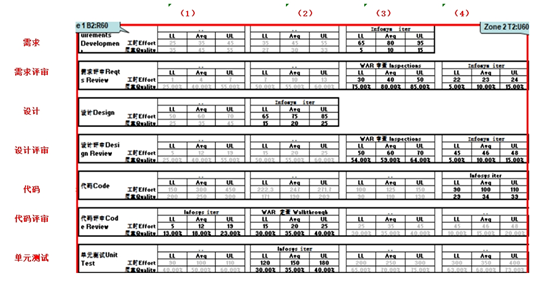
\includegraphics[width=10cm]{Sjb-1-1.png}

表13-1

%\href{文件:4reworkByPhaseScreenshot_2021-12-01_214838.1.jpg}{450px}

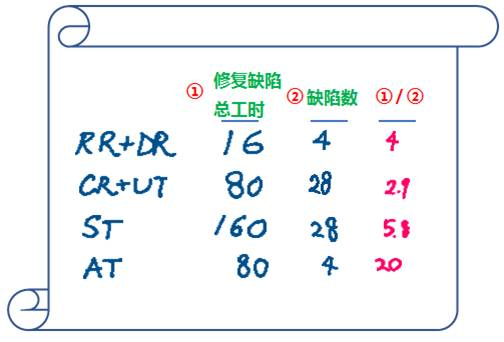
\includegraphics[width=10cm]{4reworkByPhaseScreenshot_2021-12-01_2148381.jpg}

图13-4

C/从团队工时表估算各过程的缺陷返工工作量。例如最下面一行Quality那行输入：\$20,000
(因为验收测试缺陷平均修复工时是20，假定每工时成本为
\$1,000）；系统测试那行：\$5,800(因为系统测试缺陷平均修复工时是5.8）。

%\href{文件:微信截图_20231031153355.png}{450px}


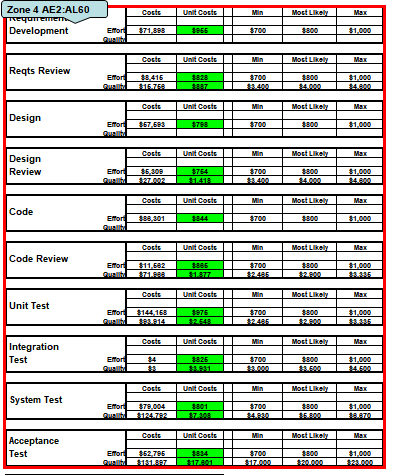
\includegraphics[width=10cm]{微信截图_20231031153355.png}

图13-5

D/
质量总成本：水晶球会依据质每过程的缺陷分布和单位成本分布，预估质量成本的分布。

\begin{description}
\item[]
\begin{description}
\tightlist
\item[]
质量总成本 +
工作（如评审，设计、开发、测试等）成本（注），得出总成本分布。
\end{description}

注：指具体做评审、测试等活动的工作量，填在模板里工时 Effort 那行
\end{description}

从水晶球得出总成本分布的95百分位数(95\% percentile) 为：\$905,022

E/ 团队分析根因后，团队找出以下3条改进建议：

\begin{enumerate}
\tightlist
\item
  用正式专家评审加强需求评审，估计能把缺陷排除率从本来10\% 提高到80\%
\item
  用评审检查单加强设计评审，估计能把缺陷排除率从本来10\% 提高到59\%
\item
  用检查单加强代码评审，估计能把缺陷排除率从本来18\% 提高到35\%
\end{enumerate}

\begin{itemize}
\tightlist
\item
  问题1：用了这些新方法会对缺陷分布有什么改善效果？
\item
  问题2：是否3种改善都使用? 或只用其中2种更有效？ （总成本最低）
\end{itemize}

把3种新方法和\%按下表加入模板：水晶球会依据质每过程的缺陷分布和单位成本分布，预估质量成本的分布。

\begin{enumerate}
\tightlist
\item
  按本来迭代需求引入缺陷数=10（3）
\item
  \textbf{需求评审缺陷排除率= 80\%}（3），需求评审缺陷排除率= 10\%（4）
\item
  设计引入缺陷数=20（2）
\item
  \textbf{设计评审排除率=59\%}（3），设计评审排除率=10\%（4）
\item
  代码引入缺陷数=34（4）
\item
  代码评审排除率=18\%（1），\textbf{代码评审排除率=35\%}（2）
\item
  单元测试缺陷排除率=35\%（2）
\item
  系统测试缺陷排除率=88\%（1）
\item
  验收测试缺陷排除率=99\%（3）
\end{enumerate}

最佳搭配是只选 加强 设计与代码评审，需求评审不变。\\
改进后成本分布的95百分位数(95\% percentile) 为：\$874,854

\begin{itemize}
\tightlist
\item
  如果我们把优化后的缺陷分布与本来迭代的缺陷分布比较，能看出改进后，本来在系统测试才发现的缺陷大多数可以预先在评审暴露，降低返工工作量，也可以预估评审缺陷范围，如果实际评审缺陷数未能达到范围，便可预警，尽快纠正\\
\end{itemize}

如果没有预测模型，我们只能主观估计会降低，有了预测模型，便可以估计缺陷分布的变化，也能帮我们挑选最佳搭配，并预估下一轮的缺陷分布范围。

%\href{文件:MTKL.png}{450px}

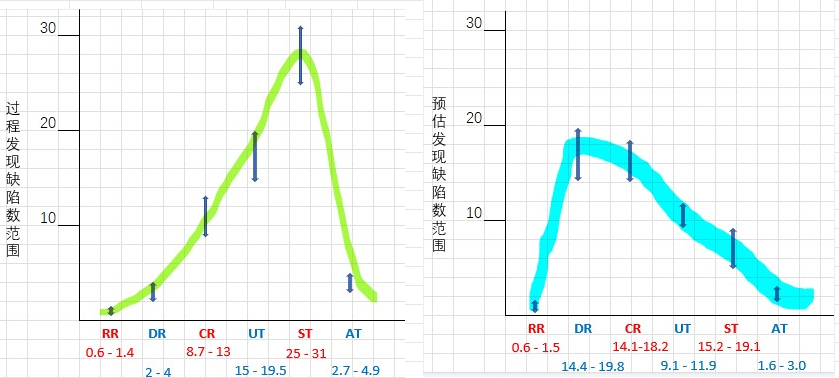
\includegraphics[width=10cm]{MTKL.png}

图13-6

\textbf{解读预测模型最佳搭配选择：}\\
模型以总成本最低可以防止局部最优。例如需求评审没有选用排除率高的新方法，因为新方法会使用较大评审工作量。如果用质量最优（质量成本最低）便必然会读选用缺陷排除率最高的方法，但用总成本来比较便可以综合考虑工作量(Effort)和质量(Quality)，避免局部最优。\\

由于不同项目甚至不同迭代冲刺的缺陷数和缺陷率各异，难以进行比较，但如果方法和团队人员相似，缺陷排除率应该是可比的。
通过分析以往的缺陷数据，针对最薄弱的环节讨论根本原因，并在下一个迭代中进行改进，提升缺陷排除率，并可以预估各个阶段（如评审、测试等）的缺陷发现数。例如，如果需求评审的缺陷数远低于预期，就应立即进行纠正，而不是像以前那样仅仅提醒大家要重视评审工作。

\begin{description}
\tightlist
\item[]
= = = =
\end{description}

\hypertarget{ux600eux6837ux5f00ux59cb}{%
\section{怎样开始}\label{ux600eux6837ux5f00ux59cb}}

一天的培训，可以帮助他们了解根因分析的重点。

%\href{文件:微信截图_20230830093612-2.jpg}{500px}

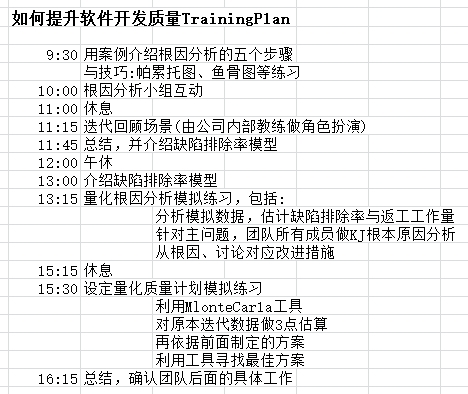
\includegraphics[width=10cm]{微信截图_20230830093612-2.jpg}

图13-7

让团队了解以下重点：\\
\textbf{改进目标}：降低返工工作量（同时也会降低缺陷后期才被发现的数量）\\
\textbf{分析根因}：不仅要分析后期发现缺陷的分类与数量，还需对从需求到最终客户验收的全生命周期进行缺陷排除率分析，以找出最薄弱的环节并深入挖掘根因。利用数据进行互动练习是最有效的学习方式，因此建议从以往的缺陷数据中抽取70-150条进行小组分析。\\
\textbf{预测效果}：以福特8D根因分析框架为例，缺陷排除与返工预测模型可以帮助团队预估新方法的效果（例如，通过代码静态扫描加强代码评审）。

团队在开始从定性到定量管理的时候，可以在回顾时，分析刚刚迭代的缺陷排除率和缺陷引入，以前没有这种细化的数据，根因分析可能只看到系统测试缺陷的总数多少，用了这个排除率的分解，就可以让团队了解主要问题来自哪里，针对性分析根因和对应措施。例如发现大部分的缺陷来自代码，就深入地去看代码出了什么问题，那一类代码缺陷比较多，针对这一类的缺陷讨论原因，下一轮做对应改进措施，并制定新一轮的量化目标。\\
量化回顾也让团队成员了解到自己的问题，更了解自己的质量和水平。

\hypertarget{ux5982ux4f55ux80fdux7b80ux5355ux6709ux6548ux5730ux6536ux96c6ux7f16ux7801ux7f3aux9677ux4e0eux8fd4ux5de5ux5de5ux4f5cux91cfux6570ux636e}{%
\subsection{如何能简单有效地收集编码缺陷与返工工作量数据}\label{ux5982ux4f55ux80fdux7b80ux5355ux6709ux6548ux5730ux6536ux96c6ux7f16ux7801ux7f3aux9677ux4e0eux8fd4ux5de5ux5de5ux4f5cux91cfux6570ux636e}}

最有效项目数据的方法就是每次迭代回顾时，同时看看本迭代缺陷的相关数据，这样团队立马可分析本迭代收集的数据（而非团队收集数据，让公司数据专员做分析）。
很多团队说"我们都有评审代码，但问题都直接改正了，没有记录。``\\
后面便不知道有多少缺陷，无法量化分析。如果要求开发人员按系统测试缺陷记录方式，在缺陷管理系统里面一条一条记，大家会觉得太花时间不愿意做。
可以利用工具帮助，例如可利用GIT做代码评审记录，也可以在GIT系统里面跟踪评审问题。不需要把问题另外记在系统测试缺陷跟踪系统，但每条问题在GIT系统里都有痕迹。开发就可以从中数出大概共有多少代码评审缺陷。如果平常也记录了每天所花的时间，他用来修改bug的工作量也有统计数据了。\\
\textbf{团队自己收集数据}：此外，团队成员应开始每天或每周自行统计返工的工作量（包括评审缺陷，所有数据均记录在缺陷管理系统中）。\\
%\href{文件:缺陷表4.1.jpg}{500px}

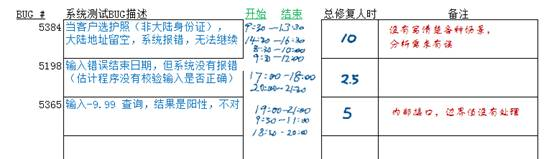
\includegraphics[width=10cm]{缺陷表41.jpg}

表13-2

建议每人自己每天记录当天工时花在什么地方，比如花在缺陷的修复的是多少。迭代结束回顾时，每人看看自己的记录。团队迭代回顾时，因为在系统里面也有评审缺陷的跟踪也可以数出来缺陷是多少，从而可以算到平均一个缺陷花多少返工工时。这样就不会要开发人员花太多时间做记录，但回顾还可以收集到开发过程的所需数据。

\hypertarget{ux4eceux8fedux4ee3ux590dux76d8ux5230ux6301ux7eedux6539ux8fdb}{%
\subsection{从迭代复盘到持续改进}\label{ux4eceux8fedux4ee3ux590dux76d8ux5230ux6301ux7eedux6539ux8fdb}}

当某些团队已经能做好回顾和根因分析，也能利用数据改善下一轮的开发质量时，如何将这种做法转变为团队或公司的持续改进呢？

\framebox{%
\begin{minipage}[t]{0.97\columnwidth}\raggedright

深圳有一家公司专门从事内部 IT 服务，因为对质量要求严格，新版本在正式投产（发版）前必须通过测试验收。公司每两周进行一次发版，并对发版成功率进行统计。因为都做了很久，依据以往水平，要求发版成功率不会低于93%，并一直都监控这个百分比趋势。某月，发现成功率跌到了92%，这引发了质量改进组启动根因分析。他们首先确认是哪个部门的问题导致发版成功率下降。后来发现有两个部门的表现最差，于是针对这两个部门进行根因分析，也对一些原因实施了纠正措施，如培训和评审等。做以后发现确实那些问题解决了。通过这些措施，问题得以解决，发版成功率也提升了，到了96%。后面他们把这个作为新的基线下限，提升至一个新的水平。

（如想更了解这案例的数据变化，详见第24章里‘控制图的应用’）

\strut
\end{minipage}}

虽然个别项目组的迭代回顾能够有效改善质量，但这些成果仅仅是高层关注下的``种子''。尽管通过工作量和缺陷的改善能够显著减少持续浪费，但如果高层不关注并投入资源，那么这些``改善''可能只是短暂的闪光，很快大家就会回到以前的工作状态。\\
反之，如公司把过程改进当成项目来管理，定目标，定期监控，便能像以上案例形成标杆（基线），而且会像上台阶一样逐步提升。\\
注意：
开始时，各团队水平不同，一般难以形成公司级标杆，但可以先形成项目组自己的标杆。

\hypertarget{ux603bux7ed3}{%
\subsection{总结}\label{ux603bux7ed3}}

有数据才可以谈改进，但收集数据花精力，所以必须有针对性，二八原则可以帮助识别应针对哪方面入手。软件开发应，软件开发团队花最多工作量的不是编码本身，用于修复缺陷工作量最多。软件开发有个特点，缺陷越后暴露，返工工作量越多，例如如果缺陷在客户使用后才暴露，可能总共要花20\textasciitilde{}50人时修正，但如果缺陷能在前面评审或单元测试发现和改正，就不会超过1人时。但很多团队，大部分缺陷都是在系统测试或验收时才暴露，前面评审、单元测试发现的缺陷都很少。

虽然很多团队的根因分析用了帕里拖图、鱼骨图的方式，这些都是基于主观判断的方式，没有真正利用基于事实的数据，而且很容易受从众心理影响，变成项目经理的一言堂，无法挖掘出真正原因，使用便利贴KJ方式可以帮团队，更好从事实总结出背后的主因。

团队所有成员一起，包括需求、开发、测试、项目经理等一起分析迭代的缺陷数据，可以计算迭代的缺陷注入和缺陷排除率，利用蒙地卡洛预测模型就可以把本来只是定性的一个改进目标变成定量，也可以满足CMMI4级的主要实践（详见附件）。

\hypertarget{ux9644ux4ef6}{%
\section{附件}\label{ux9644ux4ef6}}

\hypertarget{ux5982ux4f55ux5bf9ux5e94-cmmi-ml4-ux8981ux6c42}{%
\subsection{如何对应 CMMI ML4
要求}\label{ux5982ux4f55ux5bf9ux5e94-cmmi-ml4-ux8981ux6c42}}

\hypertarget{mpm-4.4-ux4f7fux7528ux7edfux8ba1ux4e0eux5176ux4ed6ux91cfux5316ux6280ux672fux6765ux5efaux7acbux548cux5206ux6790ux8fc7ux7a0bux6027ux80fdux6a21ux578bux5e76ux4fddux6301ux66f4ux65b0}{%
\subsubsection{MPM 4.4
使用统计与其他量化技术来建立和分析过程性能模型并保持更新}\label{mpm-4.4-ux4f7fux7528ux7edfux8ba1ux4e0eux5176ux4ed6ux91cfux5316ux6280ux672fux6765ux5efaux7acbux548cux5206ux6790ux8fc7ux7a0bux6027ux80fdux6a21ux578bux5e76ux4fddux6301ux66f4ux65b0}}

其他必需信息 Additional Required Information

\begin{description}
\tightlist
\item[]
PPM 过程性能模型：
\end{description}

\begin{itemize}
\tightlist
\item
  是根据历史过程性能数据（如过程性能基线中包含的数据）开发的

  \begin{itemize}
  \tightlist
  \item
    依据每一个过程需求评审，开发，等系统导出数据，依据数据中的缺陷建立的模型
  \end{itemize}
\item
  以可度量的属性值和术语描述、描绘变动或对其进行建模

  \begin{itemize}
  \tightlist
  \item
    有一个度量定义表，蒙特卡洛中的变量定义在度量定义表中定义;变量与预测结果都有分布
  \end{itemize}
\item
  预测中间或最终过程性能

  \begin{itemize}
  \tightlist
  \item
    蒙特卡洛可以预测出QPPO范围与过程（如需求评审）缺陷范围
  \end{itemize}
\item
  估算预测结果的预期范围和变动

  \begin{itemize}
  \tightlist
  \item
    蒙特卡洛预测出中间或最终过程QPPO的预期范围和变动
  \end{itemize}
\item
  包含至少一个表示与子过程相关的可控输入的可度量属性

  \begin{itemize}
  \tightlist
  \item
    可控因素：各阶段的评审方法（如，用走查 或 审查）
  \end{itemize}
\end{itemize}

\begin{itemize}
\tightlist
\item
  Establish PPM - Monte Carlo analysis
\item
  Validate PPM - build PPM using historical iteration defect escape
  data, check and calibrate with the recent iteration defect results
\item
  Review PPM with affected stakeholders - whole team review in Sprint
  retrospective
\item
  Revise PPM - team review and revise (if needed) the PPM using the
  current Sprint defect data in Sprint retrospective
\end{itemize}

\hypertarget{mpm-4.5-ux4f7fux7528ux7edfux8ba1ux4e0eux5176ux4ed6ux91cfux5316ux6280ux672fux6765ux786eux5b9aux6216ux9884ux6d4bux8d28ux91cfux4e0eux8fc7ux7a0bux6027ux80fdux76eeux6807ux7684ux5b9eux73b0ux60c5ux51b5}{%
\subsubsection{MPM 4.5
使用统计与其他量化技术来确定或预测质量与过程性能目标的实现情况}\label{mpm-4.5-ux4f7fux7528ux7edfux8ba1ux4e0eux5176ux4ed6ux91cfux5316ux6280ux672fux6765ux786eux5b9aux6216ux9884ux6d4bux8d28ux91cfux4e0eux8fc7ux7a0bux6027ux80fdux76eeux6807ux7684ux5b9eux73b0ux60c5ux51b5}}

\begin{itemize}
\tightlist
\item
  分析选定过程的变动和稳定性并解决缺陷

  \begin{itemize}
  \tightlist
  \item
    使用了方差分析和控制图
  \item
    通过趋势图，控制图判断历史数据是否作为基线，保证模型的稳定性。详见基线PPB截图。
  \item
    对各种方法进行方差分析，识别是否有显著区分
  \end{itemize}
\item
  实施必要的行动来解决在实现质量与过程性能目标方面的缺陷

  \begin{itemize}
  \tightlist
  \item
    P4 系统缺陷密度波动范围很广， 暂时不能预测，先对团队培训过程
  \end{itemize}
\item
  使用经数据校准并已确认的过程性能模型来评估质量与过程性能目标的实现进度

  \begin{itemize}
  \tightlist
  \item
    使用过程性能模型来预测下一轮冲刺的各阶段缺陷密度范围
  \end{itemize}
\item
  识别和管理与实现质量与过程性能目标有关的风险

  \begin{itemize}
  \tightlist
  \item
    利用PPM预测下一轮达到目标范围的概率
  \end{itemize}
\item
  记录并传达分析结果、决策以及确定的行动

  \begin{itemize}
  \tightlist
  \item
    把以上记录在量化项目管理计划
  \end{itemize}
\end{itemize}

\hypertarget{mpm-4.1-ux4f7fux7528ux7edfux8ba1ux4e0eux5176ux4ed6ux91cfux5316ux6280ux672fux6765ux5236ux5b9aux6301ux7eedux66f4ux65b0ux5e76ux4f20ux8fbeux53efux8ffdux6eafux5230ux4e1aux52a1ux76eeux6807ux7684ux8d28ux91cfux4e0eux8fc7ux7a0bux6027ux80fdux76eeux6807}{%
\subsubsection{MPM 4.1
使用统计与其他量化技术来制定、持续更新并传达可追溯到业务目标的质量与过程性能目标}\label{mpm-4.1-ux4f7fux7528ux7edfux8ba1ux4e0eux5176ux4ed6ux91cfux5316ux6280ux672fux6765ux5236ux5b9aux6301ux7eedux66f4ux65b0ux5e76ux4f20ux8fbeux53efux8ffdux6eafux5230ux4e1aux52a1ux76eeux6807ux7684ux8d28ux91cfux4e0eux8fc7ux7a0bux6027ux80fdux76eeux6807}}

\begin{itemize}
\tightlist
\item
  质量过程目标

  \begin{itemize}
  \tightlist
  \item
    组织: 用控制图、蒙特卡罗模型、方差分析等来分析SMART质量过程目标
  \item
    项目: 用预测模型、基线为下个冲刺预测质量过程目标
  \end{itemize}
\item
  制定中期目标以监控进度

  \begin{itemize}
  \tightlist
  \item
    项目:
    用预测模型来预测下一个冲刺的需求审查，代码审查，单元测试的缺陷密度范围
  \end{itemize}
\item
  确定并记录风险

  \begin{itemize}
  \tightlist
  \item
    使用预测模型来预测实现质量过程目标的百分比
  \end{itemize}
\item
  解决质量过程目标之间的冲突

  \begin{itemize}
  \tightlist
  \item
    预测模型使用整体成本来优化，可以平衡质量（减少化系统测试/验收测试缺陷密度）和生产率目标之间的冲突
  \end{itemize}
\end{itemize}

\hypertarget{plan-4.1-ux4f7fux7528ux7edfux8ba1ux4e0eux5176ux4ed6ux91cfux5316ux6280ux672fux6765ux5f00ux53d1ux9879ux76eeux8fc7ux7a0bux5e76ux4fddux6301ux66f4ux65b0ux4ee5ux5b9eux73b0ux8d28ux91cfux4e0eux8fc7ux7a0bux6027ux80fdux76eeux6807}{%
\subsubsection{PLAN 4.1
使用统计与其他量化技术来开发项目过程并保持更新，以实现质量与过程性能目标。}\label{plan-4.1-ux4f7fux7528ux7edfux8ba1ux4e0eux5176ux4ed6ux91cfux5316ux6280ux672fux6765ux5f00ux53d1ux9879ux76eeux8fc7ux7a0bux5e76ux4fddux6301ux66f4ux65b0ux4ee5ux5b9eux73b0ux8d28ux91cfux4e0eux8fc7ux7a0bux6027ux80fdux76eeux6807}}

\begin{itemize}
\tightlist
\item
  制定用于评价项目过程备选方案的准则

  \begin{itemize}
  \tightlist
  \item
    总成本最低。
  \end{itemize}
\item
  识别或开发可用来完成工作和实现目标的替代过程

  \begin{itemize}
  \tightlist
  \item
    模型中已进行体现，通过不同的评审方法互相替换。
  \end{itemize}
\item
  根据记录的评价标准分析和评价备选过程

  \begin{itemize}
  \tightlist
  \item
    参考蒙特卡洛Optimize 仿真选择最佳配搭。
  \end{itemize}
\item
  选择最符合准则的备选过程

  \begin{itemize}
  \tightlist
  \item
    同上，在模型中体现。
  \end{itemize}
\item
  评价无法实现项目的质量与过程性能目标的风险

  \begin{itemize}
  \tightlist
  \item
    利用PPM预测结果的分布，分析概率，
  \end{itemize}
\end{itemize}

\hypertarget{car-2.1-ux9009ux62e9ux8981ux8fdbux884cux5206ux6790ux7684ux7ed3ux679c}{%
\subsubsection{CAR 2.1
选择要进行分析的结果}\label{car-2.1-ux9009ux62e9ux8981ux8fdbux884cux5206ux6790ux7684ux7ed3ux679c}}

\begin{itemize}
\tightlist
\item
  确定哪些结果进一步分析：在迭代回顾时，对各个过程的缺陷数和遗留数进行总体分析，识别、选择关键过程来进一步分析。
\end{itemize}

\hypertarget{car-4.1-ux4f7fux7528ux7edfux8ba1ux7684ux4e0eux5176ux4ed6ux91cfux5316ux6280ux672fux5bf9ux9009ux5b9aux7ed3ux679cux8fdbux884cux6839ux672cux539fux56e0ux5206ux6790}{%
\subsubsection{CAR 4.1
使用统计的与其他量化技术对选定结果进行根本原因分析}\label{car-4.1-ux4f7fux7528ux7edfux8ba1ux7684ux4e0eux5176ux4ed6ux91cfux5316ux6280ux672fux5bf9ux9009ux5b9aux7ed3ux679cux8fdbux884cux6839ux672cux539fux56e0ux5206ux6790}}

\begin{itemize}
\tightlist
\item
  利用参考以往基线，包括缺陷排除公司的基线，项目自己的以往迭代的基线进行比较，或借用从以往项目数据建立的公司的预测模型，帮助团队找出根因。
\end{itemize}

\hypertarget{car-3.2-ux63d0ux51faux5904ux7406ux5df2ux786eux5b9aux7684ux6839ux672cux539fux56e0ux7684ux884cux52a8ux5efaux8bae}{%
\subsubsection{CAR 3.2
提出处理已确定的根本原因的行动建议}\label{car-3.2-ux63d0ux51faux5904ux7406ux5df2ux786eux5b9aux7684ux6839ux672cux539fux56e0ux7684ux884cux52a8ux5efaux8bae}}

\begin{itemize}
\tightlist
\item
  针对根因制定对应的新方法，例如新的评审方法或者开发方法，也估计这方法在缺陷排除或者缺陷数的量，加到模型中，利用模型的最优选择，比较这个新的方法可以比预计提升多少？
\end{itemize}

\hypertarget{car-4.2-ux4f7fux7528ux7edfux8ba1ux7684ux4e0eux5176ux4ed6ux91cfux5316ux6280ux672fux8bc4ux4ef7ux5b9eux65bdux7684ux884cux52a8ux5bf9ux8fc7ux7a0bux6027ux80fdux7684ux5f71ux54cd}{%
\subsubsection{CAR 4.2
使用统计的与其他量化技术评价实施的行动对过程性能的影响}\label{car-4.2-ux4f7fux7528ux7edfux8ba1ux7684ux4e0eux5176ux4ed6ux91cfux5316ux6280ux672fux8bc4ux4ef7ux5b9eux65bdux7684ux884cux52a8ux5bf9ux8fc7ux7a0bux6027ux80fdux7684ux5f71ux54cd}}

\begin{itemize}
\tightlist
\item
  在下一个迭代执行新方法，再下一轮回顾时看效果是否有提升？比模型预计的多少？并更莫地卡罗预测模型，
\end{itemize}

\hypertarget{car-3.4-ux8bb0ux5f55ux6839ux672cux539fux56e0ux5206ux6790ux548cux89e3ux51b3ux6570}{%
\subsubsection{CAR 3.4
记录根本原因分析和解决的数据}\label{car-3.4-ux8bb0ux5f55ux6839ux672cux539fux56e0ux5206ux6790ux548cux89e3ux51b3ux6570}}

\begin{itemize}
\tightlist
\item
  把这些都记录在A3报告里，作为公司的参考。
  公司级也可以从这些A3报告和相关数据判断是否可以扩大给其他项目组参考、使用。
\end{itemize}

\hypertarget{ux53c2ux8003-reference}{%
\section{参考 Reference}\label{ux53c2ux8003-reference}}

\begin{enumerate}
\tightlist
\item
  Juran, Joseph. ''Juran's Quality Handbook ''(1999) 5/e\\
\item
  Gladwell, Malcolm. ''Blink: The Power of Thinking Without Thinking ''
\end{enumerate}

